\documentclass[runningheads]{llncs}
\usepackage{graphicx}
\usepackage{geometry}
\usepackage{lastpage} 
\usepackage{fancyhdr} 
\geometry{left=2.0cm,right=2.0cm,top=2.0cm,bottom=2.0cm}

\begin{document}
\title{Massive Classification From Eigenvector: Comparing Neural Network,
	Decision Tree \& Maximum Likelihood}

\author{Hongxiang Zhang\inst{1}}

\authorrunning{Hongxiang Zhang.}

\institute{
	Research School of Computer Science	Australian National University\\
	\email{u7101924@anu.edu.au}
}
%
\maketitle
%
\begin{abstract}

Massive classification has become an increasing demand in the real world. While much existing work focuses on binary classification or general multiclassification. Multiple methods can be used for classification, for example, Neural Network, Decision Tree, and Maximum Likelihood[1]. In this paper, we focus on comparing Neural Network and traditional method that usually used in classification, and provides an answer that can solve massive classification.

Due to the amount of the dataset, We propose a different data format to shorten data reading time and various data preprocessing techniques. To find the answer that can solve the massive classification, We provide various methods for comparison, and multiple techniques to improve performance. Also, this paper concluded various techniques to avoid overfitting, which often exists in Massive classification. To reduce the problem complexity, we choose VehicleX[2] as the dataset, which contains vectors with shapes (1*2048) for each vehicle image. 

Comparing Neural Network, Decision Tree, and Maximum Likelihood, we found neural network is the best method to solve Massive classification. Compared to the traditional classification method, Neural Network has higher accuracy and strong robustness to noise.

\keywords{Massive Classification  \and Neural Network \and Decision Tree \and Maximum Likelihood.}

\end{abstract}

\section{Introduction}

Classification, as an essential task in machine learning, provides multiple applications in the real world. Faced with massive classification, the traditional method may have a poor performance with a waste of time and resources. In this paper, we compare Neural Network, Decision Tree, and Maximum Likelihood with the same dataset to show the performance in different methods.

VehicleX is a large-scale synthetic dataset with less content domain gap to real-world data which contains 1,362 vehicles. These data were created in Unity with various attributes. The benefit to using this dataset is that high degree of freedom on specific attributes and less spent on marking labels. To reduce the difficulty of this task, We are using vector data extracted by Resnet[3] from VehicleX[2], and we divided the dataset into the training set, test set, and validation set with 45,438, 15,142, and 14,936 data respectively. Each data is an eigenvector in 2048 dimensional, which represents a vehicle image. Faced with such a large-scale dataset, we used various preprocessing methods to optimize data, for example, Regularization, Rearrange sequences.

In this paper, we aim to use a different method to classify vehicle-ID which is 1,362 classes, and provide an answer that can solve massive classification. Due to the massive data and class in this task, our experimental strategy is to implement a Neural Network with fewer layers, train with train-set showing the accuracy and loss, and then evaluate with Val-set showing the accuracy and loss to evaluate the model. At the same time, implement a traditional method which train and test with the same dataset, compare the performance which performed by different methods. The result suggests that Neural Network always has a better performance than the traditional method in massive classification, but this network facing serious overfitting. Based on those findings, we conclude and apply serious techniques to avoid overfitting and improve performance.


\section{Method}
We introduce a large-scale synthetic dataset named VehicleX which has a diverse range of realistic backbone models and textures. To focus on our task, we are using an eigenvector extracted from VehicleX instead of the raw images, and a series of data processing. Also, we present three experiments, which use Neural Network, Decision Tree, and Maximum Likelihood respectively. Taken together, our experiments show a result that the best way to solve massive classification.


\subsection{Data Processing}
VehicleX has a diverse range of realistic backbone models and textures, allowing it to be able to adapt to the variance of real-world datasets[2]. In this paper, we aim to find the best method to solve massive classification.  As shown in Figure~\ref{fig1}, we use an eigenvector extracted by ResNet, which has a length of 2,048. Each eigenvector is store in one file. All data was separated into train-set, test-set, and Val-set with 45,438, 15,142, and 14,936 files respectively. To speed up file loading time, all eigenvectors read from files shaped with$(n, 2048)$, which n represents the length of each set, then save as a new CSV file. For label data, it stored as an array in which each element represent one label, each element represents one class that the eigenvector belongs to. And there are 1326 classes in total.

\begin{figure}
	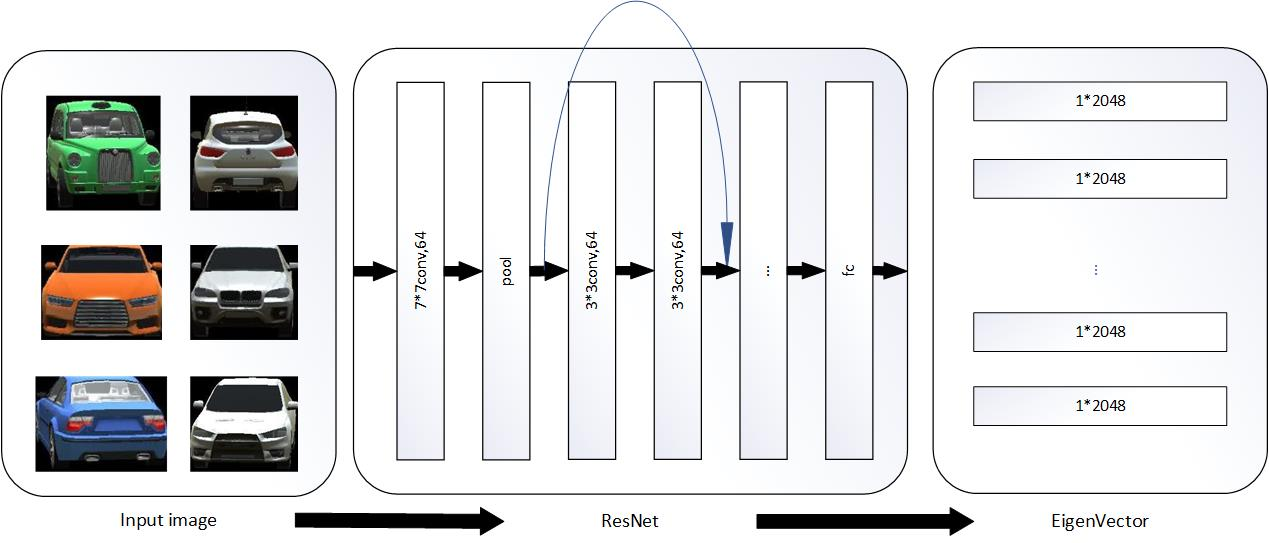
\includegraphics[width=\textwidth]{fig1.jpg}
	\caption{Illustration of the process that extracts the input eigenvectors. The first block indicates the input image, then passes it to the second block which is ResNet to extract features. The output is eigenvectors.} \label{fig1}
\end{figure}

In one eigenvector, There are 2,048 dimensions, and different dimensions have different value ranges which may have an influence on the result of classification. To reduce this influence, we use Normalization. Formally, Min-Max Normalization and Z-score Normalization are usually used for Normalization [4].

Min-Max Normalization: For each dimention $i$, the objective is map it to range $[0,1]$. $X_{max}$ represent the max value in this dimention, $X_{min}$ represent the minimum value in this dimention.
\begin{equation}
	X^i=\frac{x-X_{min}}{X_{max}-X_{min}}
\end{equation}

Z-score Normalization: For each dimension $i$, the objective is to map data to the normal distribution. $\mu$ represents the mean value in this dimension, $\sigma$ represent the standard deviation in this dimention
\begin{equation}
	X^i=\frac{x-\mu}{\sigma}
\end{equation}

In this paper, we use Min-Max Normalization to map the data into range$[0,1]$. This operation can not only reduce the bad effect of different value ranges but also Improve the convergence rate of the model. Also, Normalization makes features in different dimensions comparable, which can improve the accuracy of the classifier.

\subsection{Neural Network}
We propose a fully connected Neural Network to classify the eigenvectors into different classes. Our proposed architecture consists of two parts - a fully connected layer for learning features and a softmax layer for classification. As illustrated in Figure~\ref{fig2}, a fully connected layer takes in all input and passes the vector to the activation function which used to mapping input nonlinearly. The output of the activation function pass to the softmax layer for classification. A fully connected layer(FC)[5] is well-known for its superb performance in classification, and a Fully connected layer can map the eigenvector learned by the convolutional layer to the label space. Softmax layer generally used in multi-classification, which mapping the input to range $[0,1]$ of each category. The output of softmax can be regarded as the probability of each category, which used for classification.

\begin{figure}
	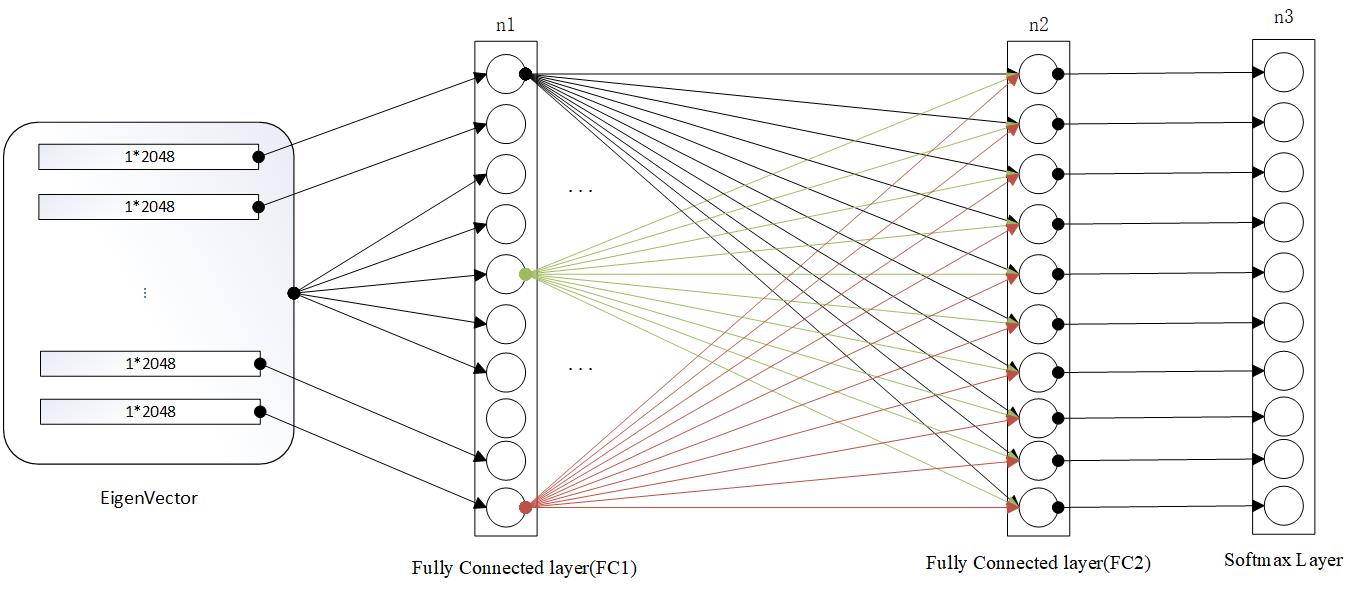
\includegraphics[width=\textwidth]{fig2.jpg}
	\caption{The neural network architecture considered in this paper. n1 stands for the number of neurons in FC1 which is the number of eigenvectors, n3 stands for the numbers of neurons in softmax layer which is the number of classification} \label{fig2}
\end{figure}

\subsubsection{Fully connected layer}
Each fully connected layer consists mulitple neurals. As illustrated in Figure 2, fully connected layer takes all eigen vectors as input, each dimension in eigen vector correspoding to one neurals. These two Fully connected layer are denoted as $FC_1$ and $FC_2$ with $n_1$ and $n_2$ neurals respectively. Assume x be one ouput of layer$FC_1$, where $x belongs to R^{{n_1}*1}$. And $W$ be the weight matrix of $FC_2$, where $W belongs to R^{{n_1}*{n_2}}$. Each colum $w_i$ in $W$ is the weight vector correspoding to $i$th neuron in $FC_2$. In this case, $W^T*x$ is the output of $FC_2$. This operation can synthesize the features extracted from the upper layers. 

\subsubsection{Activation Function}
The activation function is a nonlinear function that can enhance the neural network. As an essential part of the neural network, we compare several different activation functions: Relu, sigmoid, and leakyRelu[6]. Shown with Figure~\ref{fig3}.

As the most well-known Activation Function, sigmoid can map the input to range $(0,1)$. However, it may lead to a gradient explosion or gradient disappearance.
\begin{equation}
	f(z)=\frac{1}{1+e^(-z)}
\end{equation}

Compare to the sigmoid function, Relu computes faster and When the input is positive Relu will not have trouble with gradient explosion. However, when input is negative Relu can not be activated which called Dead Relu. In backpropagation, The gradient goes to 0 when input is negative.
\begin{equation}
	f(z)=max(0,x)
\end{equation}

To solve Dead Relu, Leaky Relu was proposed. When the input is negative, Leaky Relu still responds to the input.
\begin{equation}
	f(z)=max(\alpha x,x)
\end{equation}

\begin{figure}
	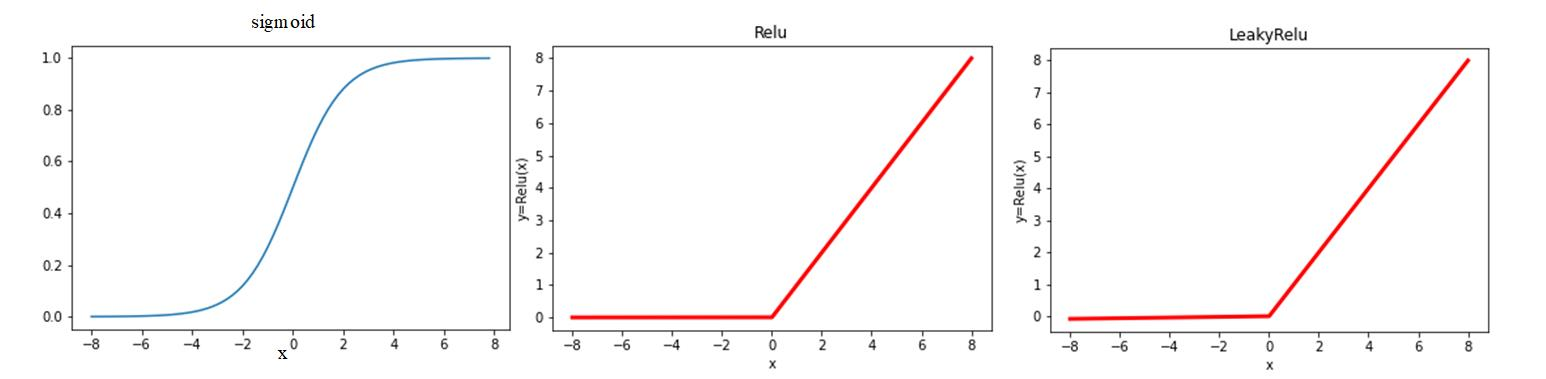
\includegraphics[width=18cm]{fig3.jpg}
	\caption{Three graph represent the activation function graph corresponding to sigmoid, Relu and LeakyRelu respectively} \label{fig3}
\end{figure}

\subsubsection{Softmax layer}
Softmax layer widely used in multi-classification, which mapping the input to range $[0,1]$ of each category. It can be regarded as the probability of each category, which used for classification. As illustrated in Figure~\ref{fig4}. Assume $V$ is the input vector of softmax layer, $z_i$ represent the $i$th category value in $V$, the output of the $i$th category is $y_i$.
\begin{equation}
	y_i=\frac{e^{z_i}}{\sum_j e^{z_j}}
\end{equation}

\begin{figure}
	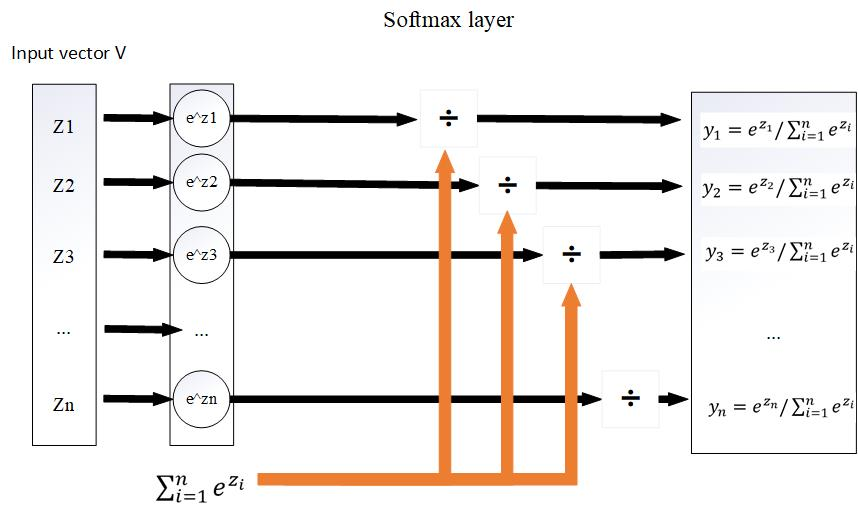
\includegraphics[width=15cm]{fig4.jpg}
	\caption{Illustration of the softmax calculation process. After calculation, each input is map to range$[0,1]$.} \label{fig4}
\end{figure}



\subsection{Decision Tree}
A Decision Tree is a divide and conquers method to classification, which widely used in discover features in a large dataset. Decision Tree uses the branch structure to classify each eigen vector into categories[7]. Shannon[8] introduces Entropy which represents the amount of eliminating the uncertainty. It was written as
\begin{equation}
	Entropy(t)=-\sum_{i=0}^{c-1}p(i|t)\log_2p(i|t)
\end{equation}
Which $p(i|t)$ represents the probability that node t belongs to class i. When the uncertainty is greater, It needs a larger amount of information and greater entropy. Also, Higher entropy represents lower purity which means when the dataset is evenly mixed, the entropy is the greatest with the lowest purity. In this paper, we build a decision tree based on purity. ID3 algorithm is an effective way to improve purity, which calculates entropy in each node. Written as
\begin{equation}
	Gain(D,a)=Entropy(D)-\sum_{i=1}^{k}\frac{|D|}{|D_i|}Entropy(D_i)
\end{equation}



\subsection{Maximum Likelihood}
Maximum Likelihood classification is a statistically based method derived from Bayes theorem, which is commonly used in traditional classification. It mainly uses a discriminant function to classify each pixel to the class with the highest likelihood [9]. This paper uses each eigen value in an eigen vector to identity the eigen vector to the corresponding class. Let $P(i|\omega)$ as the posterior distribution, $i$ is the $i$th class, $\omega$ is the feature vector.
\begin{equation}
	P(i|\omega)=\frac{P(\omega|i)P(i)}{P(\omega)}
\end{equation}
$P(\omega|i)$represent the likelihood function, and $P(i)$ is a priori information. In this case, The probility of $\omega$ is

\begin{equation}
	P(\omega)=\sum_{i=1}^{M}P(\omega|i)P(i)
\end{equation}

\section{Results and Discussion}
In this paper, we separate the dataset into trainset, test-set, and Val-set with lengths 45438, 15142, 14936 respectively. 60\% of identities are used for training, 20\% for testing, the other 20\% are used for adjusting parameters. The challenge in this data set is that the massive amount of data. To apply our model, all data are being normalized and rearrange the order then convert to the tensor which boosts computing. Normalization is an essential way that making data in different dimensions comparable and rearrange the order in some way can avoid overfitting. And in this paper, we also use CUDA to accelerated computing. To compare the performance of the three classification methods, we train the model with the same train-set and evaluate with the same test-set.

\subsection{Neural Network}
\subsubsection{Network Architectural}
For Neural Network, we compare different layers and different optimization methods to find the best network structure, then evaluate it with a Decision Tree and Maximum Likelihood. In this task, we evaluate the network in 1, 2, and 3 layers. For one layer network, it consists of an input layer with 45438 neurons and an output layer with 1362 neurons. The two-layer network consists of an input layer with 45438 neurons, an activation function layer, a hidden layer with 1600 neurons, and an output layer with 1362 neurons in order. And the three-layer network contains an input layer, two hidden layers,s and one output layer with 45438,1800,1600,1362 neurons respectively. All there network sets hyperparameter with learning rate, epochs, and optimizer as 0.001, 301, Adam. Table~\ref{tab1} gives a summary of all Three networks. 

\begin{table}
	\caption{Comparesion between 1,2 and 3 layer network}\label{tab1}
	\begin{center}
		\begin{tabular}{|l|l|l|}
			\hline
			Network & Train set Accurcy & Test set Accurcy\\
			\hline
			One layer &  {82.25\%} & 11.94\%\\
			Two layer &  {69.1\%} & 12.40\%\\
			Three layer & {44.86\%} & 11.57\%\\
			\hline
		\end{tabular}
	\end{center}
\end{table}

\begin{figure}
	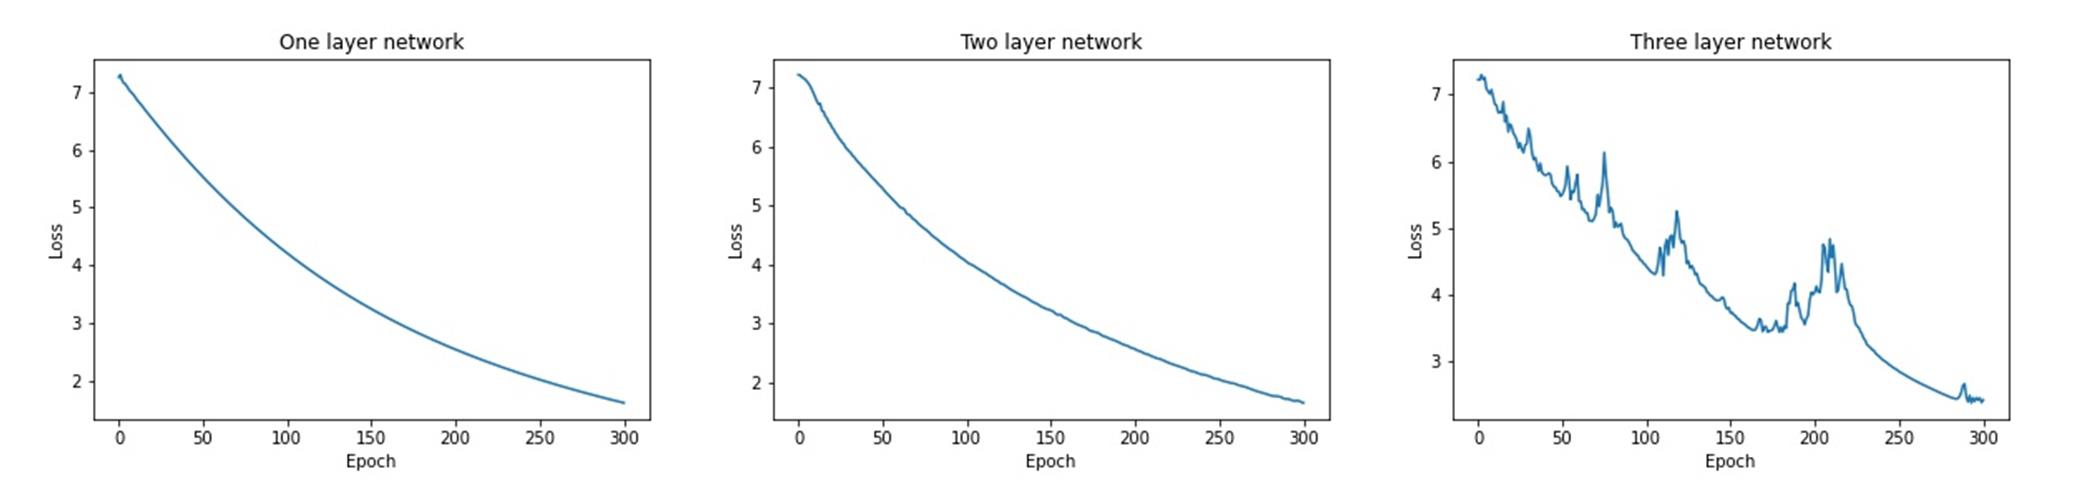
\includegraphics[width=18cm]{fig5.jpg}
	\caption{Three graph shows the curve of loss to epoch corresponding to one layer, two-layer, and three-layer network. All models run with the same dataset and same epochs.} \label{fig5}
\end{figure}

As the table~\ref{tab1} and Figure~\ref{fig5} shown, a Two-layer network has the best performance among those three network structural. And it is easy to understand why, for the network with fewer layers, it is insufficient to classify the massive classification relation clearly, so it goes to overfitting the label data in an extreme way. In this session, we found that when the neural network is deeper, the loss is not monotonic decreasing but appearing multiple wave crest which means the network is too complex to adjust the parameters well. And it is an interesting task which we can explore in the future.
\subsubsection{Hyperparameters}
Hyperparameters play an important role in a neural network, different Hyperparmaters lead a diverse performance in a model. In this session, we compare different Learning rates, epochs, and optimizers to find the best Hyperparmaters in this task. We choose a two-layer model in the last session. Table~\ref{tab2} gives a summary of choosing Hyperparmaters. 

\begin{table}
	\caption{Comparesion between Learning rate, epoches and optimiser}\label{tab2}
	\begin{center}
		\begin{tabular}{|l|l|l|l|l|}
			\hline
			Learning rate & Epoches & Optimiser & Train set Accurcy & Test set Accurcy\\
			\hline
			0.01  & 201 & SGD  & 0.06\%  & 0.05\%\\
			0.01  & 201 & Adam & 0.37\%  & 0.26\%\\
			0.01  & 301 & SGD  & 0.10\%  & 0.09\%\\
			0.01  & 301 & Adam & 1.03\%  & 0.59\%\\
			0.01  & 501 & SGD  & 0.13\%  & 0.09\%\\
			0.01  & 501 & Adam & 2.41\%  & 1.63\%\\
			\hline
			0.005 & 201 & SGD  & 0.06\%  & 0.06\%\\
			0.005 & 201 & Adam & 17.67\%  & 7.35\%\\
			0.005 & 301 & SGD  & 0.10\%  & 0.09\%\\
			0.005 & 301 & Adam & 25.92\%  & 9.52\%\\
			0.005 & 501 & SGD  & 0.08\%  & 0.04\%\\
			0.005 & 501 & Adam & 15.75\%  & 5.83\%\\
			\hline
			0.001 & 201 & SGD  & 0.07\%  & 0.09\%\\
			0.001 & 201 & Adam & 49.18\%  & 11.82\%\\
			0.001 & 301 & SGD  & 0.06\%  & 0.05\%\\
			0.001 & 301 & Adam & 69.32\%  & 12.40\%\\
			0.001 & 501 & SGD  & 0.06\%  & 0.05\%\\
			0.001 & 501 & Adam & 93.32\%  & 11.88\%\\
			\hline
		\end{tabular}
	\end{center}
\end{table}

From the table above, hyperparameters with 0.001 learning rate, 301 epoch, and Adam for optimizer is the best setting for this model. Compare Adam[10] and SGD[11], Model use SGD has a large loss and a low accuracy which indicate underfitting. Due to the stochastic character, SGD converges slower than other gradients descends method, and it may oscillate at the saddle point. In contrast, Adam combines RMSprop and Momentum, which auto-adjust learning rate and add momentum to the direction of gradient descend to speed up gradient descent. Learning rate is one of the most important hyperparameters in this paper, As Figure~\ref{fig6} illustrate, When the learning rate is 0.01, Average Loss always keep at a high level, which indicates learning rate is too high that gradient always descent overhead and it can not reach the minimum point. Compare 0.005 and 0.001, 0.005 is too high for this task, after 300 epochs, the loss is still large, It needs more epochs to reach the minimum point, which costs more time and resources. For 0.001 learning rate, the loss descent smoothly, At the end of 300 epochs, the performance is the best among those settings.
\begin{figure}
	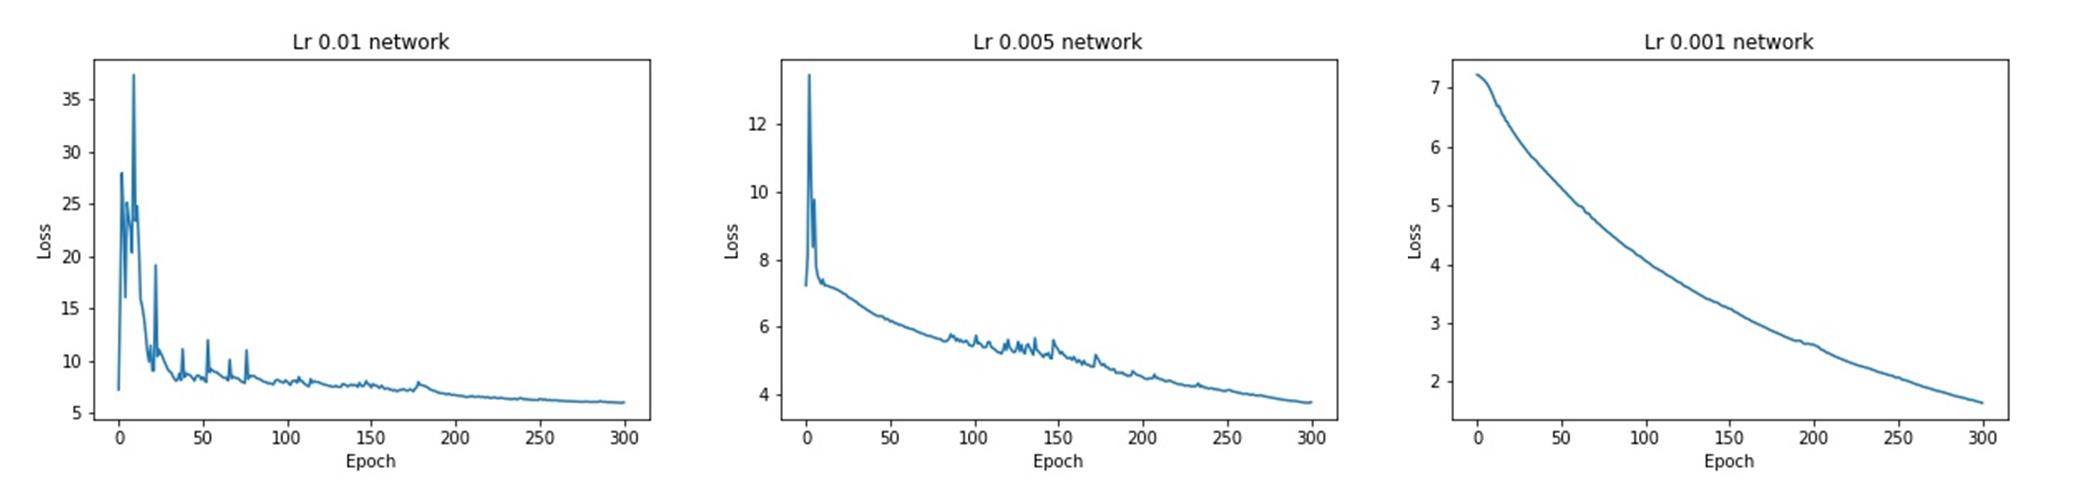
\includegraphics[width=18cm]{fig6.jpg}
	\caption{Three graph shows the curve of loss to epoch corresponding to 0.01 learning rate, 0.005 learning rate, 0.001 learning rate two-layer network. All models run with the same dataset and same epochs.} \label{fig6}
\end{figure}

\subsection{Dropout layer}
From the performance shown above, the model is overfitting. To reduce overfitting, we add a dropout layer to this model and evaluate the performace[12].

\begin{table}
	\caption{Comparesion between different dropout}\label{tab3}
	\begin{center}
		\begin{tabular}{|l|l|l|}
			\hline
			dropout probility & Train set Accurcy & Test set Accurcy\\
			\hline
			0    & 69.32\%  & 12.24\%\\
			0.3  & 49.68\%  & 9.77\%\\
			0.5  & 36.18\%  & 7.78\%\\
			\hline
		\end{tabular}
	\end{center}
\end{table}

From the table~\ref{tab3} illustrate. The dropout layer can reduce overfitting to some degree, but it also loses some useful information in the network which leads to a worse performance.
\subsection{Decision Tree}
In this task, we choose the ID3 algorithm to build a Decision Tree for classification. Due to the massive class in this paper, the Decision tree in this task has a huge amount of branches for decisions. As shown in the table~\ref{tab4}, It is unusual to achieve better performance on this dataset. Due to the Massive amount of classes, this decision tree is much complex and redundant, which means there is a small difference between each class, which leads to a bad performance on the Decision tree. In this case, our conclusion is that the Decision Tree is not a proper method for massive classification.

\begin{table}
	\caption{Decision Tree Performance }\label{tab4}
	\begin{center}
		\begin{tabular}{|l|l|l|l|}
			\hline
			          & Correct & False & Accuracy\\
			\hline
			Train set &  5707  &   39731   & 12.56\% \\
			Test set  &  67    &   15075   & 0.44\%\\
			\hline
		\end{tabular}
	\end{center}
\end{table}

\subsection{Maximum Likelihood}
For Maximum Likelihood, we choose Multinomial Naive Bayes for classification, which assumes probability distribution obeys a multinomial. For this massive classification task, we need to calculate the prior probability and conditional probability of each data to each class, then using these probabilities to estimate the class. As the table~\ref{tab5} shown, Multinomial Naive Bayes did not perform well on both the training set and test set. We can infer that simple Multinomial Naive Bayes can not fully learn the features in the dataset for classification.

\begin{table}
	\caption{Maximum Likelihood Performance }\label{tab5}
	\begin{center}
		\begin{tabular}{|l|l|l|l|}
			\hline
			& Correct & False & Accuracy\\
			\hline
			Train set &  5707  &   39731   & 29.00\% \\
			Test set  &  67    &   15075   & 6.00\%\\
			\hline
		\end{tabular}
	\end{center}
\end{table}

Kibriya, A. M., Frank, E., Pfahringer, B., \& Holmes, G. (2004, December). Multinomial naive bayes for text categorization revisited. In Australasian Joint Conference on Artificial Intelligence (pp. 488-499). Springer, Berlin, Heidelberg.

\subsection{Summary and Discussion}
After comparing Neural Network, Decision tree, and Maximum likelihood. We found that a Neural network is the best method for massive classification. In the previous experiments, we have discussed different architectural and hyperparameters. Results show that a two-layer network is the best model, which is able to classify the massive dataset and not too complicated architecture. For hyperparameters, we evaluate different hyperparameter combinations to find the best. However, as performance showed, the two-layer model is still overfitting. And we have established serious techniques to reduce overfitting, such as normalization, dropout, and rearrange the order. But it can not solve overfitting from the source. The reason why those methods are not efficient is that those techniques drop information in the network to avoid overfitting which leads to worse performance in this paper. Due to the massive class of this dataset, the key to solve overfitting is to extend the dataset. When we classify a smaller label such as vehicle type which is 10 types classification, the model reaches a marvelous performance which reaches over 93\% accuracy. In this case, sufficient data plays a key role in massive classification.

The traditional methods like Decision trees and maximum likelihood did not achieve ideal performance. The Decision tree produces the worse results on both train-set and test-set. Facing massive classification, the Decision tree needs a number of branches to classify each data which is low efficiency and bad performance. The maximum likelihood which based on statistical theory can have a good performance on normal classification, and due to the shortage of dataset, maximum likelihood performed not well.
\section{Conclusion and Future Work}
In this paper, we evaluate three methods for classification. First, we developed different architecture in the Neural network. These models are trained and evaluated with the same dataset. After the experiment, we found 2-layer Neural Network performs best, which achieves 12.40\% accuracy. After comparing the three methods, results show that the Neural Network model outperforms compared to the traditional methods. While in this paper, we also discuss different ways to optimize the model, though the network did not reach the ideal performance finally. But there still amount of ways to improve the performance, extended dataset, deeper network.

Due to the limitation of computer performance, there are also other models and techniques for classification, such as speed up SVM algorithm[13], which achieve great performance on massive classification. We will explore those techniques in the future.


\section{Reference}

\quad[1] Milne, L. K., Gedeon, T. D., \& Skidmore, A. K. (1995). Classifying Dry Sclerophyll Forest from Augmented Satellite Data: Comparing Neural Network, Decision Tree \& Maximum Likelihood. training, 109(81), 0.\\

[2] Yao, Y., Zheng, L., Yang, X., Naphade, M., \& Gedeon, T. (2019). Simulating content consistent vehicle datasets with attribute descent. arXiv preprint arXiv:1912.08855.\\

[3] He, K., Zhang, X., Ren, S., \& Sun, J. (2016). Deep residual learning for image recognition. In Proceedings of the IEEE conference on computer vision and pattern recognition (pp. 770-778).\\

[4] Jayalakshmi, T., \& Santhakumaran, A. (2011). Statistical normalization and back propagation for classification. International Journal of Computer Theory and Engineering, 3(1), 1793-8201.\\

[5] Ma, W., \& Lu, J. (2017). An equivalence of fully connected layer and convolutional layer. arXiv preprint arXiv:1712.01252.\\

[6] Ramachandran, P., Zoph, B., \& Le, Q. V. (2017). Searching for activation functions. arXiv preprint arXiv:1710.05941.\\

[7] Myles, A. J., Feudale, R. N., Liu, Y., Woody, N. A., \& Brown, S. D. (2004). An introduction to decision tree modeling. Journal of Chemometrics: A Journal of the Chemometrics Society, 18(6), 275-285.\\

[8] Bromiley, P. A., Thacker, N. A., \& Bouhova-Thacker, E. (2004). Shannon entropy, Renyi entropy, and information. Statistics and Inf. Series (2004-004).\\

[9] Strahler, A. H. (1980). The use of prior probabilities in maximum likelihood classification of remotely sensed data. Remote sensing of Environment, 10(2), 135-163.\\

[10] Kingma, D. P., \& Ba, J. (2014). Adam: A method for stochastic optimization. arXiv preprint arXiv:1412.6980.\\

[11] Bottou, L. (2010). Large-scale machine learning with stochastic gradient descent. In Proceedings of COMPSTAT'2010 (pp. 177-186). Physica-Verlag HD.\\

[12] Baldi, P., \& Sadowski, P. J. (2013). Understanding dropout. Advances in neural information processing systems, 26, 2814-2822.\\

[13] Do, T. N., Nguyen, V. H., \& Poulet, F. (2008, October). Speed up the SVM algorithm for massive classification tasks. In International conference on advanced data mining and applications (pp. 147-157). Springer, Berlin, Heidelberg.
\end{document}
